
\documentclass[english, a4paper, 12pt]{report}
\usepackage[T1]{fontenc}
\usepackage[latin1]{inputenc}
\usepackage[english]{babel}
\usepackage{fullpage}
\usepackage{color}
\usepackage{graphics, graphicx}
\usepackage{wrapfig}
\usepackage{natbib}
\usepackage{algorithm2e}
\usepackage{amsmath}
\usepackage{amssymb}
\usepackage{caption}
\usepackage{bookmark}
\usepackage{lineno}
\usepackage{hyperref}
\usepackage{pdfpages}

\hypersetup{
    backref=true,
    pagebackref=true,
    hyperindex=true,
    colorlinks=true,
    breaklinks=true,
    urlcolor=black,
    linkcolor=black,
    citecolor=black,
    bookmarks=true,
    bookmarksopen=true,
    pdffitwindow=true,
    pdfauthor={Charles Rocabert},
    pdftitle={},
    pdfsubject={},
    pdfcreator={charles.rocabert@gmail.com},
    pdfkeywords={}
}

% Define environnement tablehere
\renewcommand{\textfraction}{0}
\makeatletter
\newenvironment{tablehere}
{\def\@captype{table}}
{}

% Define environnement figurehere
\newenvironment{figurehere}
{\def\@captype{figure}}
{}
\makeatother

% Define some variables
\newcommand{\packageName}{\textsc{Evo\textsuperscript{2}Sim}}
\newcommand{\packageVersion}{1.0.2}

\begin{document}
%\selectlanguage{english}

%%%%%% TITLE PAGE %%%%%%

\thispagestyle{empty}

\rule{\linewidth}{2pt}
\begin{figure}[!h]
\centering
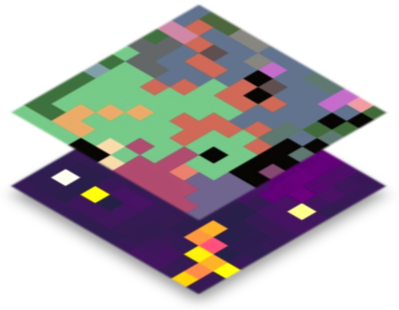
\includegraphics[width=0.2\linewidth]{./figures/icon.png}
\end{figure}

\begin{center}
{\Huge {\bf {\packageName} User Manual}}

for version {\packageVersion} (\today)
\end{center}
\rule{\linewidth}{2pt}

\newpage

\tableofcontents

\newpage

%%%%%%%%%%%%%%%%%%%

\chapter{Introduction}

\section{Introducing \packageName}

{\packageName} is a multi-scale model of \textit{in silico} experimental evolution, the virtual pendant of experimental evolution in wet laboratory (see Fig~\ref{general_algorithm}).
The software is equiped with the whole tool case of experimental setups, competition assays, phylogenetic analysis, and, most importantly, allowing for evolvable ecological interactions. Digital organisms with an evolvable genome structure, encoding evolvable genetic regulation and metabolic networks are evolved for tens of thousands of generations in environments mimicking the dynamics of real controlled environments, including chemostat or batch culture.

{\packageName} was developed under \textsc{EvoEvo} (\href{http://www.evoevo.eu/}{http://www.evoevo.eu/}), a project funded by the European Commission (FP7-ICT-610427, FET-Proactive: Evolving Living Technologies). The source code is written in C++.

You shall find more details on the software and its development on the Github repository https://github.com/charlesrocabert/{\packageName}.

\section{License}

This program is free software: you can redistribute it and/or modify it under the terms of the GNU General Public License as published by the Free Software Foundation, either version 3 of the License, or (at your option) any later version.

This program is distributed in the hope that it will be useful, but WITHOUT ANY WARRANTY; without even the implied warranty of MERCHANTABILITY or FITNESS FOR A PARTICULAR PURPOSE. See the GNU General Public License for more details.

You should have received a copy of the GNU General Public License along with this program. If not, see \href{http://www.gnu.org/licenses/}{http://www.gnu.org/licenses/}.

\section{Community}
{\packageName} was developed by Charles Rocabert, Carole Knibbe and Guillaume Beslon, under the \textsc{EvoEvo} project. The list of contributors is displayed in text-file \texttt{AUTHORS} of {\packageName}  package.
You shall find more details on \href{http://www.evoevo.eu/community/}{http://www.evoevo.eu/community/}.

\section{Download}
{\packageName} last releases are freely available on the Github repository\\https://github.com/charlesrocabert/{\packageName}.

\section{Contact}
For any question about the software, do not hesitate to contact us at\\ \href{http://www.evoevo.eu/contact-us/}{http://www.evoevo.eu/contact-us/}.

\newpage
\thispagestyle{empty}

\begin{figurehere}
\centering 
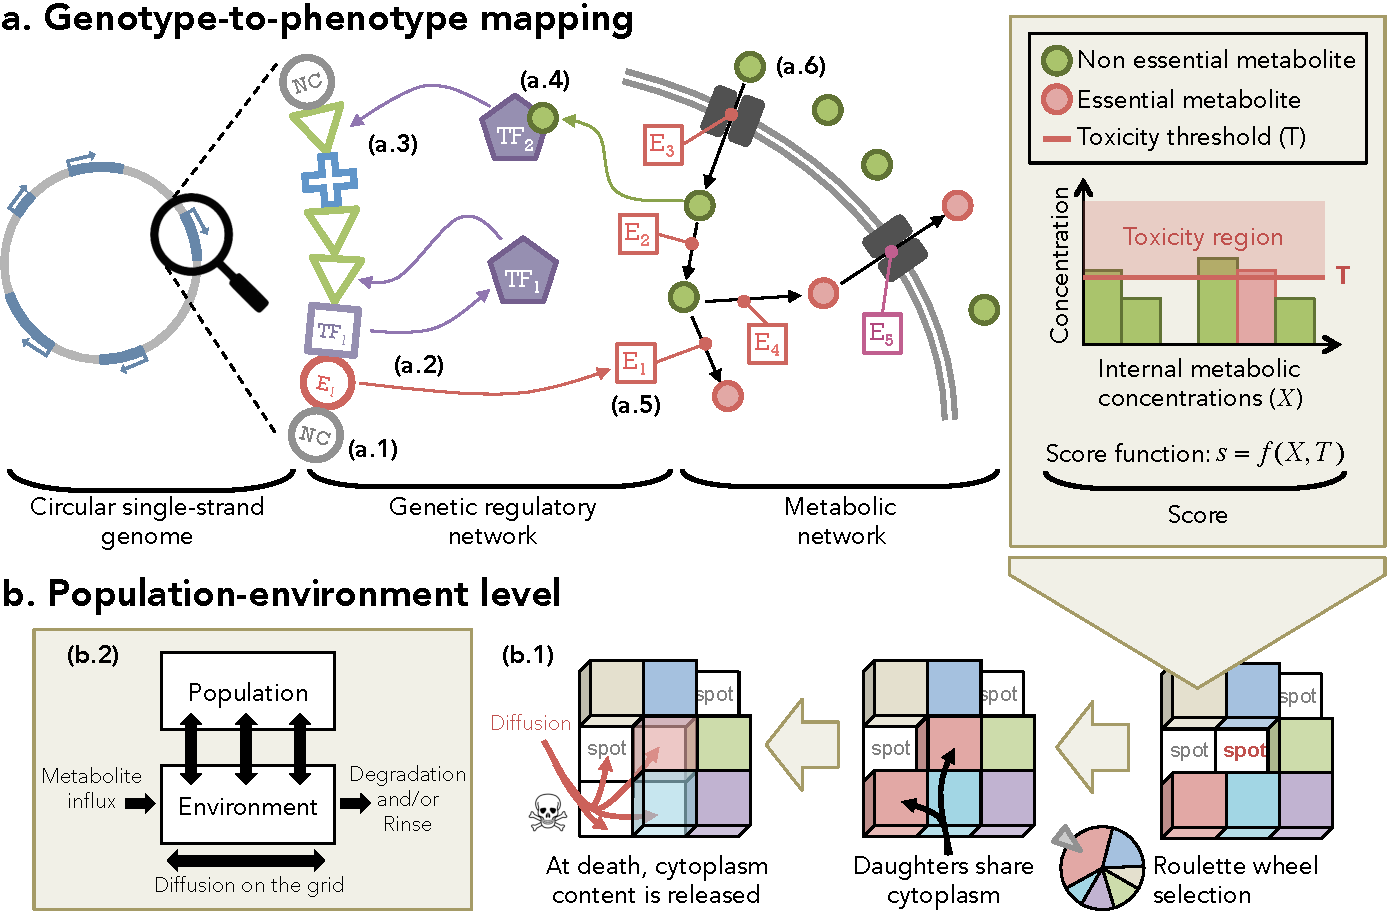
\includegraphics[width=0.95\textwidth]{figures/general_algorithm.pdf}
\caption[Global picture of {\packageName}.]{\small{\textbf{Global picture of {\packageName}.} \textbf{a. Description of the genotype-to-phenotype mapping.} Organisms own a coarse-grained genome made of units. This genome is a circular single-strand sequence, with a unique reading frame. Non coding \textbf{(NC)} units are not functional \textbf{(a.1)}. The arrangement of the units on the sequence defines functional regions, where a promoter (\textbf{P}, blue cross) controls the expression of enzyme coding units (\textbf{E}, red circles) or transcription factor coding units (\textbf{TF}, purple squares), thereby allowing for operons (here, one E and one TF). When coding units are expressed \textbf{(a.2)}, they contribute to the genetic regulatory network (for TFs) and the metabolic network (for Es).
Depending on their attributes, transcription factors bind on binding sites. \textbf{(a.3)} If they bind on the enhancer sequence (binding sites flanking the promoter upstream), the promoter activity is up-regulated. If they bind on the operator sequence (binding sites flanking the promoter downstream), the promoter activity is down-regulated. \textbf{(a.4)} Metabolites can bind on a transcription factor as co-enzymes, and activate or inhibit it, depending on transcription factor attributes.
Enzymes perform metabolic reactions in the cytoplasm \textbf{(a.5)}, or pump metabolites in or out \textbf{(a.6)}. The score of an organism is computed from its ``essential metabolites''
(usually the score is the sum of essential metabolite concentrations). Lethal toxicity thresholds are applied to each metabolic concentration and forbid organisms to accumulate resources. \textbf{b. Description of the population and environment levels.} Organisms are placed on a 2D toroidal grid, and compete for resources and space. When an organism dies, it leaves its grid cell empty and organisms in the Moore neighborhood (if any) compete to divide in available space. The competition is based on scores, a minimal threshold being applied on scores to forbid worst organisms to divide. At division, daughters share cytoplasm content (enzymes and metabolites). At death, metabolites from the cytoplasm are released in the local environment, and diffuse on the grid \textbf{(b.1)}. On the largest scale, the population evolves on the environment by up-taking, transforming and releasing metabolites. Metabolites then diffuse and are degraded. This strong interaction between the population and the environment allows for the evolution of complex ecological situations, depending on environmental properties \textbf{(b.2)}.}}
\label{general_algorithm}
\end{figurehere}




\chapter{Installation instructions}

Download the latest release of {\packageName} on Github page charlesrocabert/Evo2Sim and save it to a directory of your choice. Open a terminal and use the \texttt{cd} command to navigate to this directory. Then follow the steps below to compile and build the executables.

\section{Supported platforms}
{\packageName} software has been successfully tested on Ubuntu 12.04 LTS, Ubuntu 14.04 LTS, OSX 10.9.5 (Maverick) and OSX 10.10.1 (Yosemite).

\subsection{Required dependencies}
\begin{itemize}
	\item A \texttt{C++} compiler (GCC, LLVM, ...)
	\item \texttt{CMake} (command line version)
	\item \texttt{zlib}
	\item \texttt{GSL}
	\item \texttt{CBLAS}
	\item \texttt{TBB}
	\item \texttt{R} (packages \texttt{ape} and \texttt{RColorBrewer} are needed)
\end{itemize}

\subsection{Optional dependencies (for graphical outputs)}
\begin{itemize}
	\item \texttt{X11} (or \texttt{XQuartz} on latest OSX version)
	\item \texttt{SFML 2}
	\item \texttt{matplotlib} (this python library is needed for the script \texttt{track\_cell.py} (see below)
\end{itemize}

\subsection{HTML viewer dependencies}
\begin{itemize}
	\item Javascript must be activated in your favorite internet browser
\end{itemize}

Note, however, that {\packageName} can be compiled without graphical outputs, and hence no need for X and SFML libraries (see compilation instructions below for more information). This option is useful if you want to run {\packageName} on a computer cluster, for example.

\section{Software compilation}

\subsection{User mode}
To compile {\packageName}, run the following instructions on the command line:
\begin{itemize}
	\item[\$] \texttt{cd cmake/}
\end{itemize}
and
\begin{itemize}
	\item[\$] \texttt{bash make.sh}
\end{itemize}

To gain performances during large experimental protocols, or on computer cluster, you should compile the software without graphical outputs:
\begin{itemize}
	\item[\$] \texttt{bash make\_no\_graphics.sh}
\end{itemize}

\subsection{Debug mode}
To compile the software in \texttt{DEBUG} mode, use \texttt{make\_debug.sh} script instead of \texttt{make.sh}:
\begin{itemize}
	\item[\$] \texttt{bash make\_debug.sh}
\end{itemize}
When {\packageName} is compiled in \texttt{DEBUG} mode, a lot of tests are computed on the fly during a simulation (\textit{e.g.} integrity tests on phylogenetic trees, or on the ODE solver \ldots). For this reason, this mode should only be used for test or development phases. Moreover, unitary and integrated tests must be ran in \texttt{DEBUG} mode (see below).

\subsection{Executable files emplacement}
Binary executable files are in \texttt{build/bin} folder.


\chapter{Typical usage}

{\packageName} includes three main executables (\texttt{evo2sim\_create}, \texttt{evo2sim\_bootstrap} and \texttt{evo2sim\_run}), and a set of executables dedicated to post-treatments, data recovery or tests.

Everything in {\packageName} relies on an ad-hoc file organization where all the data for a simulation is stored: populations in the \texttt{population} directory, environments in \texttt{environment}, phylogenetic and lineage trees in \texttt{tree} and so on. It is not recommended to manually modify these files since this may cause some inconsistency leading to undefined behavior. Besides, most of these files are compressed.

Open a terminal and use the \texttt{cd} command to navigate to {\packageName} directory.
A typical parameters file is provided in {\packageName} package, in folder \texttt{example} (an exhaustive description of the parameters is available in chapter ``Parameters description''). Navigate to this folder using the \texttt{cd} command.
Then follow the steps below for a first usage of the software.

\section{Creating a simulation}

Create a fresh simulation from the parameters file (by default \texttt{parameters.txt}):
\begin{itemize}
        \item[\$] \texttt{../build/bin/evo2sim\_create}
\end{itemize}
Several folders have been created. They mainly contain simulation backups (population, environment, trees, parameters, ...). Additional files and folders have also been created:
\begin{itemize}
        \item \texttt{version.txt}: this file indicates the version of the software. This information is useful to ensure that the code version is compatible with the backup files (\textit{e.g.}, in case of post-treatments).
        \item \texttt{track\_cell.py}: when executed, this python script displays on the fly the internal protein and metabolic concentrations of the cell at position $0\times0$ on the grid. This script is useful to get an idea of internal cell's dynamics (metabolic fluxes, regulation, \ldots).
        \item \texttt{viewer} folder: the viewer is central to the usage of {\packageName} (see chapter ``Simulation viewer''). To access the viewer, open the html page \texttt{viewer/viewer.html} in an internet browser.
\end{itemize}

\section{Generating viable initial conditions with a bootstrap}

Alternatively to the \texttt{evo2sim\_create} executable, use a bootstrap to find a simulation with good initial properties from the parameters file:
\begin{itemize}
        \item[\$] \texttt{../build/bin/evo2sim\_bootstrap}
\end{itemize}
A fresh simulation with an updated parameters file will be automatically created if a suitable seed is found.

\section{Running a simulation}

In {\packageName}, running a simulation necessitates to load it from backup files. Here, we will run a simulation from freshly created backups (see above):
\begin{itemize}
        \item[\$] \texttt{../build/bin/evo2sim\_run -b 0 -t 10000 -g}
\end{itemize}
with \texttt{-b} the date of the backup, here 0 (fresh simulation), \texttt{-t} the simulation time, here 10,000 time-steps. Option \texttt{-g} activates the graphical output (not works if the software has been compiled with the no-graphics option).
At any moment during the simulation, you can take a closer look at the evolution of the system by opening \texttt{viewer/viewer.html} in an internet browser. You can track internal cell's dynamics by executing the script \texttt{track\_cell.py}.

Other main executables are described below in section ``Main executables description''. You can also obtain help by running the executable with the \texttt{-h} option (e.g. \texttt{evo2sim\_create -h})


\chapter{Simulation viewer}

{\packageName} comes with an HTML viewer displaying a very complete set of live statistics. Each new simulation owns a dedicated viewer, which is frequently actualized on the fly (by default, every 500 simulation time-steps). This viewer has been developed using \texttt{Bootstrap}, \texttt{DyGraph}, \texttt{CytoscapeJS}, \texttt{ChartJS} and \texttt{JQuery}.

To access the viewer, simply open \texttt{viewer/viewer.html} in an internet browser (Javascript must be enabled). The different tabs are described below.

\section{Population} 
This page displays the evolution of main population statistics (population size, mean genome size, mean score, ...), as well as the evolution of the trophic network.

\section{Best lineage}
This page displays the evolution of last best individual statistics. These informations are the most representative of evolutionary dynamics, since they contains all the mutations fixed since the beginning of the simulation.

\section{Best individual}
This page displays some informations about the last best individual at the moment of the visualization (genome state, genetic regulation network, metabolic network, internal metabolic state, ...).

\section{Environment}
This page displays the evolution of main environment statistics, as well as its current state.

\section{Phylogeny}
This page displays various rendering of the current phylogenetic tree, as well as some evolution statistics (number of nodes, common ancestor age, ...).

\section{Parameters}
This page displays the parameters file used to create the simulation, as well as a short description of parameters usage.


\appendix

\chapter{Main executables description}

%================= CREATE ====================
\section{\texttt{evo2sim\_create} executable}
Create a fresh simulation from a parameters file.
\paragraph{Usage:}
\begin{itemize}
        \item[\$] \texttt{evo2sim\_create -h} or \texttt{-{}-help}
        \item[or]
        \item[\$] \texttt{evo2sim\_create [options]}
\end{itemize}
\paragraph{Options are:}
\begin{description}
        \item[\texttt{-h, -{}-help}:] print this help, then exit (optional)
        \item[\texttt{-v, -{}-version}:] print the current version, then exit (optional)
        \item[\texttt{-f, -{}-file}:] specify the parameters file (default: \texttt{parameters.txt})
        \item[\texttt{-rs, -{}-random-seed}:] the prng seed is drawn at random (optional)
\end{description}
Be aware that creating a simulation in a folder completely erases previous simulation.

%================= BOOTSTRAP =========================
\section{\texttt{evo2sim\_bootstrap} executable}
Run a bootstrap to find viable initial conditions.
\paragraph{Usage:}
\begin{itemize}
        \item[\$] \texttt{evo2sim\_bootstrap -h} or \texttt{-{}-help}
        \item[or]
        \item[\$] \texttt{evo2sim\_bootstrap [options]}
\end{itemize}
\paragraph{Options are:}
\begin{description}
        \item[\texttt{-h, -{}-help}:] print this help, then exit (optional)
        \item[\texttt{-v, -{}-version}:] print the current version, then exit (optional)
        \item[\texttt{-f, -{}-file}:] specify the parameters file (default: \texttt{parameters.txt})
        \item[\texttt{-min, -{}-minimum-time}:] specify the minimum time the new population must survive (default: 100)
        \item[\texttt{-pop, -{}-minimum-pop-size}:] specify the minimum size the new population must maintain (default: 500)
        \item[\texttt{-t, --trials}:] specify the number of trials (default: 1000)
        \item[\texttt{-g, -{}-graphics}:]  activate graphic display (optional)
\end{description}
A simulation is automatically created if good conditions are found.
The parameters file is also edited to include the corresponding prng seed value.
Be aware that creating a simulation in a folder completely erases previous simulation.

%================= RUN =========================
\section{\texttt{evo2sim\_run} executable}
Run a simulation from backup files.
\paragraph{Usage:}
\begin{itemize}
        \item[\$] \texttt{evo2sim\_run -h} or \texttt{-{}-help}
        \item[or]
        \item[\$] \texttt{evo2sim\_run [options]}
\end{itemize}
\paragraph{Options are:}
\begin{description}
        \item[\texttt{-h, -{}-help}:] print this help, then exit (optional)
        \item[\texttt{-v, -{}-version}:] print the current version, then exit (optional)
        \item[\texttt{-b, -{}-backup-time}:] set the date of the backup to load (default: 0)
        \item[\texttt{-t, -{}-simulation-time}:] set the duration of the simulation (default: 10000)
        \item[\texttt{-g, -{}-graphics}:]  activate graphic display (optional)
\end{description}
Statistic files content is automatically managed when a simulation is reloaded from backup to avoid data loss.

%================= GENERATE FIGURES =========================
\section{\texttt{evo2sim\_generate\_figures} executable}
Extract statistics and generate viewer figures from backup files.
\paragraph{Usage:}
\begin{itemize}
        \item[\$] \texttt{evo2sim\_generate\_figures -h} or \texttt{-{}-help}
        \item[or]
        \item[\$] \texttt{evo2sim\_generate\_figures [options]}
\end{itemize}
\paragraph{Options are:}
\begin{description}
        \item[\texttt{-h, -{}-help}:] print this help, then exit (optional)
        \item[\texttt{-v, -{}-version}:] print the current version, then exit (optional)
        \item[\texttt{-b, -{}-backup-time}:] set the date of the backup to load (mandatory)
\end{description}

%================= RECOVER PARAMETERS =========================
\section{\texttt{evo2sim\_recover\_parameters} executable}
Recover the parameters file from backup files.
\paragraph{Usage:}
\begin{itemize}
        \item[\$] \texttt{evo2sim\_recover\_parameters -h} or \texttt{-{}-help}
        \item[or]
        \item[\$] \texttt{evo2sim\_recover\_parameters [options]}
\end{itemize}
\paragraph{Options are:}
\begin{description}
        \item[\texttt{-h, -{}-help}:] print this help, then exit (optional)
        \item[\texttt{-v, -{}-version}:] print the current version, then exit (optional)
        \item[\texttt{-f, -{}-file}:] specify the name of the parameters file to save (mandatory)
\end{description}
    
%================= UNITARY TESTS =========================
\section{\texttt{evo2sim\_unitary\_tests} executable}
Run unitary tests.
\paragraph{Usage:}
\begin{itemize}
        \item[\$] \texttt{evo2sim\_unitary\_tests -h} or \texttt{-{}-help}
        \item[or]
        \item[\$] \texttt{evo2sim\_unitary\_tests [options]}
\end{itemize}
\paragraph{Options are:}
\begin{description}
        \item[\texttt{-h, -{}-help}:] print this help, then exit (optional)
        \item[\texttt{-v, -{}-version}:] print the current version, then exit (optional)
        \item[\texttt{-f, -{}-file}:] specify the parameters file (default: \texttt{parameters.txt})
\end{description}

To use the unitary tests, the software must be compiled in DEBUG mode (see installation instructions below).

%================= INTEGRATED TESTS =========================
\section{\texttt{evo2sim\_integrated\_tests} executable}
Run integrated tests.
\paragraph{Usage:}
\begin{itemize}
        \item[\$] \texttt{evo2sim\_integrated\_tests -h} or \texttt{-{}-help}
        \item[or]
        \item[\$] \texttt{evo2sim\_integrated\_tests [options]}
\end{itemize}
\paragraph{Options are:}
\begin{description}
        \item[\texttt{-h, -{}-help}:] print this help, then exit (optional)
        \item[\texttt{-v, -{}-version}:] print the current version, then exit (optional)
        \item[\texttt{-f, -{}-file}:] specify the parameters file (default: \texttt{parameters.txt})
        \item[\texttt{-tests, -{}-number-of-tests}:] specify the number of tests with different seeds (default: 1)
        \item[\texttt{-steps, -{}-number-of-steps}:] specify the number of steps by test (default: 1)
        \item[\texttt{-rs, -{}-random-seed}:] the prng seed is drawn at random for each test (optional)
        \item[\texttt{-rp, -{}-random-parameters}:] the parameters are drawn at random for each test (optional)
\end{description}

To use the unitary tests, the software must be compiled in DEBUG mode (see installation instructions below).

\section{Other executables}

For all the other executables, you can obtain help by running the executable with the \texttt{-h} option (e.g. \texttt{evo2sim\_create -h})





\chapter{Parameters description}

All the parameters of the parameters file are described in details below. Each parameters receive at least on value. There is three types of values:
\begin{itemize}
	\item {\bf integer}: integer number
	\item {\bf float}: floating point number
	\item {\bf string}: characters string
\end{itemize}
For each parameter, the type is possibly bounded. In this case, boundaries are indicated.

%%%%%%%%%%%%%%%%%%%%%%%%%%%%%%%%%%%%%%%%%%%%

\section{Pseudorandom numbers generator}

\begin{center}
{\bf SEED} <seed> (integer > 0)
\end{center}
Simply set the seed of the pseudorandom numbers generator (prng). The seed value is important since it allows to exactly replay a simulation if needed. 

%%%%%%%%%%%%%%%%%%%%%%%%%%%%%%%%%%%%%%%%%%%%

\section{Parallel computing}

\begin{center}
{\bf PARALLEL\_COMPUTING} <choice> (YES/NO)
\end{center}
This parameter allows to activate, or deactivate, parallel computing at will. Parallel computing is managed by the external library \texttt{TBB}.

%%%%%%%%%%%%%%%%%%%%%%%%%%%%%%%%%%%%%%%%%%%%

\section{Simulation schemes}

\subsection{Energy costs scheme}
\begin{center}
{\bf ENERGY\_COSTS\_SCHEME} <choice> (YES/NO)
\end{center}
Choose the energy scheme. By default, biochemical reactions are energy free in {\packageName}. When energy costs are activated, inner cell's chemical reactions produce or consume energy (an abstract view of energy carriers, like ATP). Transcription, enzymatic reactions and pumps else produce or cost energy to the cell, which must maintain its energy level to survive. Specific parameters are used to precisely set energy costs (see below).

%%%%%%%%%%%%%%%%%%%%%%%%%%%%%%%%%%%%%%%%%%%%

\subsection{Membrane permeability scheme}
\begin{center}
{\bf MEMBRANE\_PERMEABILITY\_SCHEME} <choice> (YES/NO)
\end{center}
Choose membrane permeability scheme. If membrane permeability is activated, metabolites diffuse through the cell's membrane at a specific rate (see MEMBRANE\_PERMEABILITY parameter below).

%%%%%%%%%%%%%%%%%%%%%%%%%%%%%%%%%%%%%%%%%%%%

\subsection{Metabolic inheritance scheme}
\begin{center}
{\bf METABOLIC\_INHERITANCE\_SCHEME} <choice> (YES/NO)
\end{center}
Choose metabolic inheritance scheme. If this parameter is activated, the two daughter cells share the metabolic content of their parent. Each daughter cell inherits half of metabolic concentrations.

%%%%%%%%%%%%%%%%%%%%%%%%%%%%%%%%%%%%%%%%%%%%

\subsection{Enzymatic inheritance scheme}
\begin{center}
{\bf ENZYMATIC\_INHERITANCE\_SCHEME} <choice> (YES/NO)
\end{center}
Choose enzymatic inheritance scheme. If this parameter is activated, the two daughter cells share the enzymatic content of their parent. Each daughter cell inherits half of enzymatic concentrations.

%%%%%%%%%%%%%%%%%%%%%%%%%%%%%%%%%%%%%%%%%%%%

\subsection{Co-enzymes scheme}
\begin{center}
{\bf CO\_ENZYME\_ACTIVITY} <choice> (YES/NO)
\end{center}
Choose co-enzyme scheme. If this parameter is activated, some metabolites act as co-enzymes. Each transcription-factor owns a site where a specific metabolite can bind, activating or inhibiting the transcription factor depending on its properties. Activating this parameter increases the complexity of the genetic regulation network, and more importantly, allows cells to evolve environmental sensing.

%%%%%%%%%%%%%%%%%%%%%%%%%%%%%%%%%%%%%%%%%%%%

\subsection{Score scheme}
\begin{center}
{\bf SCORE\_SCHEME} <choice> (SUM/SUM\_MINUS\_DEV/COMBINATORIAL)
\end{center}
Choose the score scheme. The score of a cell is computed from its internal metabolic concentrations:
\begin{itemize}
\item SUM scheme: the score is simply the sum of essential metabolite concentrations;
\item SUM\_MINUS\_DEV scheme: the score is the sum of essential metabolite concentrations, minus the standard deviation of the concentrations. This score adds an homeostatic constraint on cells.
\item COMBINATORIAL scheme: the score is computed depending on relative essential metabolite concentrations. Basically, essential metabolites are considered to form complex molecules similar to RNA polymerases. Bigger is the polymerase, higher is its contribution to the score. Then, the bigger polymerase including all the essential metabolites is defined by the lowest concentration. Since the lowest metabolite is exhausted for this polymerase, the next one is the contribution of remaining metabolites, and so forth.
\end{itemize}

%%%%%%%%%%%%%%%%%%%%%%%%%%%%%%%%%%%%%%%%%%%%

\subsection{Selection threshold}
\begin{center}
{\bf SELECTION\_THRESHOLD} <threshold> (float $\in [0, 1]$)
\end{center}
Define a score threshold, above which cell's division is forbidden. When neighboring cells compete for a gap in the environment, one cell is elected at random by a roulette wheel draw, based on relative scores. However, a minimum threshold is mandatory to avoid individuals owning a very low score to divide, and drive the population in an artificial dead-end (where everybody is very bad, but nobody dies).

%%%%%%%%%%%%%%%%%%%%%%%%%%%%%%%%%%%%%%%%%%%%

\section{Space}

\subsection{Grid width}
\begin{center}
{\bf WIDTH} <width> (integer > 0)
\end{center}
Simply define the width of the environmental grid.

%%%%%%%%%%%%%%%%%%%%%%%%%%%%%%%%%%%%%%%%%%%%

\subsection{Grid height}
\begin{center}
{\bf HEIGHT} <height> (integer > 0)
\end{center}
Simply define the height of the environmental grid.

%%%%%%%%%%%%%%%%%%%%%%%%%%%%%%%%%%%%%%%%%%%%

\section{Output}

\subsection{Simulation backup step}
\begin{center}
{\bf SIMULATION\_BACKUP\_STEP} <step> (integer $\ge 0$)
\end{center}
Define the frequency at which backups of the simulation are saved. The resolution is in simulation time-steps. It is possible to exactly replay a simulation from backup files. Be aware that backup files size is large, the backup frequency must be reasonable (\textit{e.g.}, 1,000 time-steps).

%%%%%%%%%%%%%%%%%%%%%%%%%%%%%%%%%%%%%%%%%%%%

\subsection{Figures generation step}
\begin{center}
{\bf FIGURES\_GENERATION\_STEP} <step> (integer $\ge 0$)
\end{center}
Define the frequency at which figures are generated for the html viewer. Some scripts used to generate figures may take more time to execute for very long simulations, the backup frequency must be reasonable (\textit{e.g.}, 1,000 time-steps).

%%%%%%%%%%%%%%%%%%%%%%%%%%%%%%%%%%%%%%%%%%%%

\section{Genome}

\subsection{Load the genome from file}
\begin{center}
{\bf LOAD\_GENOME\_FROM\_FILE} <choice> (YES/NO)
\end{center}
Choose to generate genomes at random (NO, in this case, random generation depends on parameters below), or load a handcrafted genome from a file (YES). In case the handcrafted genome is loaded, it must be encoded in a file named \texttt{initial\_genome.txt}. The structure of this file is specific and must respect the following scheme:
\begin{enumerate}
\item To encode non-coding units (NC), insert the following line: \texttt{NC <number of units>}. The specified number of random NC units will be inserted (\texttt{<number of units>} $> 0$);
\item To encode a promoter unit (P), insert the following line: \texttt{P <basal expression level>}. A promoter unit with a basal expression level $\beta=\texttt{<basal expression level>}$ will be inserted ($\beta \in [0,1]$);
\item To encode a binding site unit (BS), insert the following line: \texttt{BS <TF tag>}. A binding site unit owning the specified transcription factor tag value will be inserted (\texttt{<TF tag>} $\in \mathbb{Z}$);
\item To encode a transcription factor coding unit (TF), insert the following line: \texttt{TF <BS tag> <CoE tag> <free activity> <bound activity> <binding window>}. A transcription factor coding unit with specified attributes will be inserted (\texttt{<BS tag>} $\in \mathbb{Z}$, \texttt{<CoE tag>} $\in \mathbb{N}^*$, \texttt{<free activity>} $\in \{true, false\}$, \texttt{<bound activity>} $\in \{true, false\}$, \texttt{<binding window>} $\ge 0$);
\item To encode an enzyme coding unit (E), insert the following line: \texttt{E <substrate> <product> <$k_{cat}$> <$K_M$>}. An enzyme coding unit with specified attributes will be inserted (\texttt{<substrate>} $> 0$, \texttt{<product>} $> 0$, \texttt{<$k_{cat}$>} and \texttt{<$K_M$>} $\in$ specified boundaries).
\end{enumerate}

%%%%%%%%%%%%%%%%%%%%%%%%%%%%%%%%%%%%%%%%%%%%

\subsection{Metabolite tags initial range}
\begin{center}
{\bf METABOLITE\_TAG\_INITIAL\_RANGE} <min> <max> (integer > 0; min $\le$ max)
\end{center}
Define the initial distribution of metabolite tags encoded in the initial random genome (\textit{i.e.}, in transcription factor and enzyme units). \texttt{min} and \texttt{max} values define the boundaries of a uniform law, used to draw the metabolite tags.

%%%%%%%%%%%%%%%%%%%%%%%%%%%%%%%%%%%%%%%%%%%%

\subsection{Binding site tags initial range}
\begin{center}
{\bf BINDING\_SITE\_TAG\_INITIAL\_RANGE} <min> <max> (float > 0; min $\le$ max)
\end{center}
Define the initial distribution of binding site tags encoded in the initial random genome (\textit{i.e.}, in transcription factor units). \texttt{min} and \texttt{max} values define the boundaries of a uniform law, used to draw the binding site tags.

%%%%%%%%%%%%%%%%%%%%%%%%%%%%%%%%%%%%%%%%%%%%

\subsection{Co-enzyme tags initial range}
\begin{center}
{\bf CO\_ENZYME\_TAG\_INITIAL\_RANGE} <min> <max> (float > 0; min $\le$ max)
\end{center}
Define the initial distribution of co-enzyme tags encoded in the initial random genome (\textit{i.e.}, in transcription factor units). \texttt{min} and \texttt{max} values define the boundaries of a uniform law, used to draw the co-enzyme tags.

%%%%%%%%%%%%%%%%%%%%%%%%%%%%%%%%%%%%%%%%%%%%

\subsection{Transcription factor tags initial range}
\begin{center}
{\bf TRANSCRIPTION\_FACTOR\_TAG\_INITIAL\_RANGE} <min> <max> (float > 0; min $\le$ max)
\end{center}
Define the initial distribution of transcription factor tags encoded in the initial random genome (\textit{i.e.}, in binding site units). \texttt{min} and \texttt{max} values define the boundaries of a uniform law, used to draw the transcription factor tags.

%%%%%%%%%%%%%%%%%%%%%%%%%%%%%%%%%%%%%%%%%%%%

\subsection{Transcription factors binding window}
\begin{center}
{\bf TRANSCRIPTION\_FACTOR\_BINDING\_WINDOW} <window> (integer $\ge$ 0)
\end{center}
Define the ``binding window'' of a transcription factor on a binding site. If transcription factors and binding site tags are similar enough, the binding is allowed. More precisely if $\mbox{tag}_{TF} \in [\mbox{tag}_{TF}-\mbox{window}\ ,\ \mbox{tag}_{TF}+\mbox{window}]$, the binding is possible.

%%%%%%%%%%%%%%%%%%%%%%%%%%%%%%%%%%%%%%%%%%%%

\subsection{Initial number of non-coding units}
\begin{center}
{\bf INITIAL\_NUMBER\_OF\_NON\_CODING\_UNITS} <number> (integer $\ge$ 0)
\end{center}
Define the number of random non-coding units in the initial random genome.

%%%%%%%%%%%%%%%%%%%%%%%%%%%%%%%%%%%%%%%%%%%%

\subsection{Initial number of enzyme coding units}
\begin{center}
{\bf INITIAL\_NUMBER\_OF\_ENZYME\_UNITS} <number> (integer $\ge$ 0)
\end{center}
Define the number of random enzyme units in the initial random genome.

%%%%%%%%%%%%%%%%%%%%%%%%%%%%%%%%%%%%%%%%%%%%

\subsection{Initial number of transcription factor coding units}
\begin{center}
{\bf INITIAL\_NUMBER\_OF\_TRANSCRIPTION\_FACTOR\_UNITS} <number> (integer $\ge$ 0)
\end{center}
Define the number of random transcription factor units in the initial random genome.

%%%%%%%%%%%%%%%%%%%%%%%%%%%%%%%%%%%%%%%%%%%%

\subsection{Initial number of binding site units}
\begin{center}
{\bf INITIAL\_NUMBER\_OF\_BINDING\_SITE\_UNITS} <number> (integer $\ge$ 0)
\end{center}
Define the number of random binding site units in the initial random genome.

%%%%%%%%%%%%%%%%%%%%%%%%%%%%%%%%%%%%%%%%%%%%

\subsection{Initial number of promoter units}
\begin{center}
{\bf INITIAL\_NUMBER\_OF\_PROMOTER\_UNITS} <number> (integer $\ge$ 0)
\end{center}
Define the number of random promoter units in the initial random genome.

%%%%%%%%%%%%%%%%%%%%%%%%%%%%%%%%%%%%%%%%%%%%

\subsection{Point mutation rate}
\begin{center}
{\bf POINT\_MUTATION\_RATE} <rate> (float $\in [0, 1]$)
\end{center}
Define the point mutation rate (in attribute\textsuperscript{-1}.replication\textsuperscript{-1}).

%%%%%%%%%%%%%%%%%%%%%%%%%%%%%%%%%%%%%%%%%%%%

\subsection{Duplication rate}
\begin{center}
{\bf DUPLICATION\_RATE} <rate> (float $\in [0, 1]$)
\end{center}
Define the duplication rate (in genomic-unit\textsuperscript{-1}.replication\textsuperscript{-1}).

%%%%%%%%%%%%%%%%%%%%%%%%%%%%%%%%%%%%%%%%%%%%

\subsection{Deletion rate}
\begin{center}
{\bf DELETION\_RATE} <rate> (float $\in [0, 1]$)
\end{center}
Define the deletion rate (in genomic-unit\textsuperscript{-1}.replication\textsuperscript{-1}).

%%%%%%%%%%%%%%%%%%%%%%%%%%%%%%%%%%%%%%%%%%%%

\subsection{Translocation rate}
\begin{center}
{\bf TRANSLOCATION\_RATE} <rate> (float $\in [0, 1]$)
\end{center}
Define the translocation rate (in genomic-unit\textsuperscript{-1}.replication\textsuperscript{-1}).

%%%%%%%%%%%%%%%%%%%%%%%%%%%%%%%%%%%%%%%%%%%%

\subsection{Inversion rate}
\begin{center}
{\bf INVERSION\_RATE} <rate> (float $\in [0, 1]$)
\end{center}
Define the inversion rate (in genomic-unit\textsuperscript{-1}.replication\textsuperscript{-1}).

%%%%%%%%%%%%%%%%%%%%%%%%%%%%%%%%%%%%%%%%%%%%

\subsection{Transition rate}
\begin{center}
{\bf TRANSITION\_RATE} <rate> (float $\in [0, 1]$)
\end{center}
Define the transition rate  (in genomic-unit\textsuperscript{-1}.replication\textsuperscript{-1}).

%%%%%%%%%%%%%%%%%%%%%%%%%%%%%%%%%%%%%%%%%%%%

\subsection{Breakpoint rate}
\begin{center}
{\bf BREAKPOINT\_RATE} <rate> (float $\in [0, 1]$)
\end{center}
Define the breakpoint rate  (in attribute\textsuperscript{-1}.breakpoint\textsuperscript{-1}).

%%%%%%%%%%%%%%%%%%%%%%%%%%%%%%%%%%%%%%%%%%%%

\subsection{Substrate tag mutation size}
\begin{center}
{\bf SUBSTRATE\_TAG\_MUTATION\_SIZE} <size> (integer $\ge 0$)
\end{center}
Define the size of the uniform distribution used to mutate substrate tags (in enzyme units). The mutation is defined as tag + $\mathcal{U}$(-size, +size).

%%%%%%%%%%%%%%%%%%%%%%%%%%%%%%%%%%%%%%%%%%%%

\subsection{Product tag mutation size}
\begin{center}
{\bf PRODUCT\_TAG\_MUTATION\_SIZE} <size> (integer $\ge 0$)
\end{center}
Define the size of the uniform distribution used to mutate product tags (in enzyme units). The mutation is defined as tag + $\mathcal{U}$(-size, +size).

%%%%%%%%%%%%%%%%%%%%%%%%%%%%%%%%%%%%%%%%%%%%

\subsection{$k_{cat}$ mutation size}
\begin{center}
{\bf KCAT\_MUTATION\_SIZE} <size> (float $\ge 0.0$)
\end{center}
Define the standard deviation of the gaussian distribution used to mutate $k_{cat}$ constant (in enzyme units). The mutation is defined as $log_{10}(k_{cat})$ + $\mathcal{N}$(0, size).

%%%%%%%%%%%%%%%%%%%%%%%%%%%%%%%%%%%%%%%%%%%%

\subsection{$k_{cat}/k_M$ ratio mutation size}
\begin{center}
{\bf KCAT\_KM\_RATIO\_MUTATION\_SIZE} <size> (float $\ge 0.0$)
\end{center}
Define the standard deviation of the gaussian distribution used to mutate $k_{cat}/k_M$ ratio (in enzyme units). The mutation is defined as $log_{10}(k_{cat}/k_M)$ + $\mathcal{N}$(0, size).

%%%%%%%%%%%%%%%%%%%%%%%%%%%%%%%%%%%%%%%%%%%%

\subsection{Binding site tag mutation size}
\begin{center}
{\bf BINDING\_SITE\_TAG\_MUTATION\_SIZE} <size> (integer $\ge 0$)
\end{center}
Define the size of the uniform distribution used to mutate binding site tags (in transcription factor units). The mutation is defined as tag + $\mathcal{U}$(-size, +size).

%%%%%%%%%%%%%%%%%%%%%%%%%%%%%%%%%%%%%%%%%%%%

\subsection{Co-enzyme tag mutation size}
\begin{center}
{\bf CO\_ENZYME\_TAG\_MUTATION\_SIZE} <size> (integer $\ge 0$)
\end{center}
Define the size of the uniform distribution used to mutate co-enzyme tags (in transcription factor units). The mutation is defined as tag + $\mathcal{U}$(-size, +size).

%%%%%%%%%%%%%%%%%%%%%%%%%%%%%%%%%%%%%%%%%%%%

\subsection{Transcription factor tag mutation size}
\begin{center}
{\bf TRANSCRIPTION\_FACTOR\_TAG\_MUTATION\_SIZE} <size> (integer $\ge 0$)
\end{center}
Define the size of the uniform distribution used to mutate transcription factor tags (in binding site units). The mutation is defined as tag + $\mathcal{U}$(-size, +size).

%%%%%%%%%%%%%%%%%%%%%%%%%%%%%%%%%%%%%%%%%%%%

\subsection{Basal expression level mutation size}
\begin{center}
{\bf BASAL\_EXPRESSION\_LEVEL\_MUTATION\_SIZE} <size> (float $\ge 0.0$)
\end{center}
Define the standard deviation of the gaussian distribution used to mutate $\beta$ constant (in promoter units). The mutation is defined as $\beta$ + $\mathcal{N}$(0, size).

%%%%%%%%%%%%%%%%%%%%%%%%%%%%%%%%%%%%%%%%%%%%

\section{Genetic regulation network}

\subsection{Genetic regulation network time-steps ratio}
\begin{center}
{\bf GENETIC\_REGULATION\_NETWORK\_TIMESTEP} <time-step> (float > 0.0)
\end{center}
Define the number of ODE time-steps used to solve the genetic regulation network per simulation time-step.

%%%%%%%%%%%%%%%%%%%%%%%%%%%%%%%%%%%%%%%%%%%%

\subsection{Hill function theta parameter}
\begin{center}
{\bf HILL\_FUNCTION\_THETA} <theta> (float $\in [0, 1]$)
\end{center}
Define the parameter $\theta$ of the Hill function used to compute the contribution of the regulation on each promoter transcription.

%%%%%%%%%%%%%%%%%%%%%%%%%%%%%%%%%%%%%%%%%%%%

\subsection{Hill function n parameter}
\begin{center}
{\bf HILL\_FUNCTION\_N} <n> (float $\ge 0.0$)
\end{center}
Define the parameter $n$ of the Hill function used to compute the contribution of the regulation on each promoter transcription.

%%%%%%%%%%%%%%%%%%%%%%%%%%%%%%%%%%%%%%%%%%%%

\subsection{Protein degradation rate}
\begin{center}
{\bf PROTEIN\_DEGRADATION\_RATE} <rate> (float $\in [0, 1]$)
\end{center}
Define the protein degradation rate per genetic regulation ODE time-step.

%%%%%%%%%%%%%%%%%%%%%%%%%%%%%%%%%%%%%%%%%%%%

\section{Metabolic network}

\subsection{Metabolism time-steps}
\begin{center}
{\bf METABOLISM\_TIMESTEP} <time-step> (float > 0.0)
\end{center}
Define the number of ODE time-steps used to solve the metabolic network per simulation time-step.

%%%%%%%%%%%%%%%%%%%%%%%%%%%%%%%%%%%%%%%%%%%%

\subsection{Essential metabolites toxicity threshold}
\begin{center}
{\bf ESSENTIAL\_METABOLITES\_TOXICITY\_THRESHOLD} <threshold> (float > 0.0)
\end{center}
Define the maximum cell's toxicity threshold of essential metabolites. If one essential metabolite overreaches this threshold in cell's cytoplasm, the cell dies. 

%%%%%%%%%%%%%%%%%%%%%%%%%%%%%%%%%%%%%%%%%%%%

\subsection{Non-essential metabolites toxicity threshold}
\begin{center}
{\bf NON\_ESSENTIAL\_METABOLITES\_TOXICITY\_THRESHOLD} <threshold> (float > 0.0)
\end{center}
Define the maximum cell's toxicity threshold of non-essential metabolites. If one non-essential metabolite overreaches this threshold in cell's cytoplasm, the cell dies. 

%%%%%%%%%%%%%%%%%%%%%%%%%%%%%%%%%%%%%%%%%%%%

\subsection{Initial metabolite amount in cells}
\begin{center}
{\bf INITIAL\_METABOLITES\_AMOUNT\_IN\_CELLS} <initial\_amount> (float $\ge 0.0$)
\end{center}
Define the initial amount of metabolites found in cells when the simulation is created from scratch.

%%%%%%%%%%%%%%%%%%%%%%%%%%%%%%%%%%%%%%%%%%%%

\subsection{Maximum reaction size}
\begin{center}
{\bf MAXIMUM\_REACTION\_SIZE} <size> (integer $\ge 0$)
\end{center}
Define the maximum jump size of a metabolic reaction in the metabolic space. Considering $s$ and $p$ to be resp. the tags of the substrate and the product of a metabolic reaction (catalyzed by an enzyme), the reaction only occurs if $|s-p| \le \mbox{size}$.

%%%%%%%%%%%%%%%%%%%%%%%%%%%%%%%%%%%%%%%%%%%%

\section{Energy}

\subsection{Energy transcription cost}
\begin{center}
{\bf ENERGY\_TRANSCRIPTION\_COST} <cost> (float $\ge 0$)
\end{center}
Define the cost of producing proteins (mainly by transcription). When a enzyme or transcription factor unit is transcribed at a certain rate $e$, energy cost is $c = e*cost$. For computation reasons, the energy is not coupled to transcription equations (\textit{i.e.}, the reaction speed of the transcription does not depend on energy concentration). If the cost is set to 0.0, the transcription comes with no energy cost. If the energy becomes negative, the cell dies.

%%%%%%%%%%%%%%%%%%%%%%%%%%%%%%%%%%%%%%%%%%%%

\subsection{Energy degradation cost}
\begin{center}
{\bf ENERGY\_DEGRADATION\_COST} <cost> (float $\ge 0$)
\end{center}
Define the cost of degrading proteins. When proteins are degraded at rate $d$, energy cost is $c = d*cost$. For computation reasons, the energy is not coupled to degradation equations (\textit{i.e.}, the speed of the degradation does not depend on energy concentration). If the cost is set to 0.0, the degradation comes with no energy cost. If the energy becomes negative, the cell dies.

%%%%%%%%%%%%%%%%%%%%%%%%%%%%%%%%%%%%%%%%%%%%

\subsection{Energy enzymatic cost}
\begin{center}
{\bf ENERGY\_ENZYMATIC\_COST} <cost> (float $\ge 0$)
\end{center}
Define the cost or the production of energy when performing metabolic reactions. Metabolic reactions are performed by enzymes needing or producing energy carrier molecules. Let's consider $s$ and $p$ the tags of resp. the substrate and the product of a metabolic reaction catalyzed by enzyme $E$. If $s < p$, the reaction consumes energy at rate $c = (p-s)*cost$. If $s > p$, the reaction produces energy at rate $c = (s-p)*cost$. For computation reasons, the energy is not coupled to metabolic reaction equations (\textit{i.e.}, the reaction speed does not depend on energy concentration). If the cost is set to 0.0, metabolic reactions come with no energy cost. If the energy becomes negative, the cell dies.

%%%%%%%%%%%%%%%%%%%%%%%%%%%%%%%%%%%%%%%%%%%%

\subsection{Energy pumping cost}
\begin{center}
{\bf ENERGY\_PUMPING\_COST} <cost> (float $\ge 0$)
\end{center}
Define the cost of pumping in or out metabolites. When metabolites are pumped in or out at rate $r$ by a pump, energy cost is $c = r*cost$. For computation reasons, the energy is not coupled to pump equations (\textit{i.e.}, the reaction speed does not depend on energy concentration). If the cost is set to 0.0, the pumping activity comes with no energy cost. If the energy becomes negative, the cell dies.

%%%%%%%%%%%%%%%%%%%%%%%%%%%%%%%%%%%%%%%%%%%%

\subsection{Energy dissipation rate}
\begin{center}
{\bf ENERGY\_DISSIPATION\_RATE} <rate> (float $\in [0, 1]$)
\end{center}
Define the rate at which a cell looses its energy stock by dissipation.

%%%%%%%%%%%%%%%%%%%%%%%%%%%%%%%%%%%%%%%%%%%%

\subsection{Energy toxicity threshold}
\begin{center}
{\bf ENERGY\_TOXICITY\_THRESHOLD} <threshold> (float $\ge 0$)
\end{center}
Define a maximum threshold to cell's energy. If a cell energy stock overreaches this threshold, the cell dies.

%%%%%%%%%%%%%%%%%%%%%%%%%%%%%%%%%%%%%%%%%%%%

\subsection{Initial energy amount in cells}
\begin{center}
{\bf INITIAL\_ENERGY\_AMOUNT\_IN\_CELLS} <amount> (float $\ge 0$)
\end{center}
Define the initial energy amount available in cells when the simulation is created from scratch. This parameter allow for random initialization of complex cells needing energy production to survive.

%%%%%%%%%%%%%%%%%%%%%%%%%%%%%%%%%%%%%%%%%%%%

\section{Cell}

\subsection{Membrane permeability}
\begin{center}
{\bf MEMBRANE\_PERMEABILITY} <permeability> (float $\in [0, 1]$)
\end{center}
Define the membrane permeability. Metabolites in cell's cytoplasm or in the local environment diffuse through the cell's membrane depending on their concentrations and the permeability.

%%%%%%%%%%%%%%%%%%%%%%%%%%%%%%%%%%%%%%%%%%%%

\section{Population}

\subsection{Death probability}
\begin{center}
{\bf DEATH\_PROBABILITY} <probability> (float $\in [0, 1]$)
\end{center}
Define the probability to die at random per simulation time-step. This probability is the same for every cell, and is constant during cell life. This rate is applied in addition to other death events linked to toxicity thresholds.

%%%%%%%%%%%%%%%%%%%%%%%%%%%%%%%%%%%%%%%%%%%%

\subsection{Migration rate}
\begin{center}
{\bf MIGRATION\_RATE} <rate> (float $\in [0, 1]$)
\end{center}
If the migration rate is not null, pairs of random cells exchange their location at a defined rate per simulation time-step. Depending on the strength of the random mixing, cell's behavior evolve differently (\textit{e.g.}, to evolve cooperation).

%%%%%%%%%%%%%%%%%%%%%%%%%%%%%%%%%%%%%%%%%%%%

\subsection{HGT rate}
\begin{center}
{\bf HGT\_RATE} <rate> (float $\in [0, 1]$)
\end{center}
Define the probability for a genome to receive alien genetic sequences at replication. Genetic sequences are generated at random, and do not come from the simulated population.

%%%%%%%%%%%%%%%%%%%%%%%%%%%%%%%%%%%%%%%%%%%%

\section{Environment}

\subsection{Environment initialization cycles}
\begin{center}
{\bf ENVIRONMENT\_INITIALIZATION\_CYCLES} <cycles> (integer $\ge 0$)
\end{center}
Define the number of initialization loops applied to a newly created environment. Initialization loops are based on environment parameters defined below. For example, If a concentration $c = 0.1$ of metabolite $10$ is introduced in the environment at every simulation time-step, and if 5 initialization cycles are requested, the initial concentration will be $0.1 \times 5$. This parameter is useful to allow the environment to reach dynamic equilibrium before introducing new cells.

%%%%%%%%%%%%%%%%%%%%%%%%%%%%%%%%%%%%%%%%%%%%

\subsection{Environment species tags range}
\begin{center}
{\bf ENVIRONMENT\_SPECIES\_TAG\_RANGE} <min> <max> (integer > 0; min $\le$ max)
\end{center}
Define the boundaries of the uniform law used to draw a new metabolite introduced in the environment.

%%%%%%%%%%%%%%%%%%%%%%%%%%%%%%%%%%%%%%%%%%%%

\subsection{Environment concentrations range}
\begin{center}
{\bf ENVIRONMENT\_CONCENTRATION\_RANGE} <min> <max> (float > 0.0; min $\le$ max)
\end{center}
Define the boundaries of the uniform law used to draw the concentration of each new metabolite introduced in the environment.

%%%%%%%%%%%%%%%%%%%%%%%%%%%%%%%%%%%%%%%%%%%%

\subsection{Environment number of species range}
\begin{center}
{\bf ENVIRONMENT\_NUMBER\_OF\_SPECIES\_RANGE} <min> <max> (integer > 0.0; min $\le$ max)
\end{center}
Define the boundaries of the uniform law used to draw the number of metabolites introduced in the environment.

%%%%%%%%%%%%%%%%%%%%%%%%%%%%%%%%%%%%%%%%%%%%

\subsection{Environment interaction scheme}
\begin{center}
{\bf ENVIRONMENT\_INTERACTION\_SCHEME} <choice> (NO\_INTERACTION/INTERACTION)
\end{center}
Define the interaction scheme between the population and the environment.
\begin{itemize}
\item NO\_INTERACTION: environment concentrations are not modified by cells. Cells grow on ressources with constant concentrations.
\item INTERACTION: cells modify their environment by uptaking or releasing food.
\end{itemize}

%%%%%%%%%%%%%%%%%%%%%%%%%%%%%%%%%%%%%%%%%%%%

\subsection{Environment renewal scheme}
\begin{center}
{\bf ENVIRONMENT\_RENEWAL\_SCHEME} <choice> (KEEP\_MATTER/CLEAR\_MATTER)
\end{center}
Define the renewal scheme of the environment at each new variation.
\begin{itemize}
\item CLEAR\_MATTER: the environment is rinsed at each variation.
\item KEEP\_MATTER: the environment is NOT rinsed at each variation.
\end{itemize}

%%%%%%%%%%%%%%%%%%%%%%%%%%%%%%%%%%%%%%%%%%%%

\subsection{Environment variation scheme}
\begin{center}
{\bf ENVIRONMENT\_VARIATION\_SCHEME} <choice> (RANDOM/PERIODIC/CYCLIC)
\end{center}
Define the variation scheme of the environment.
\begin{itemize}
\item PERIODIC: variation periodically occurs with frequency INTRODUCTION\_RATE
\item RANDOM: variation occurs with probability INTRODUCTION\_RATE
\item CYCLIC: variation occurs at each time-step, but is pondered by a sinus function of period 1/INTRODUCTION\_RATE
\end{itemize}

%%%%%%%%%%%%%%%%%%%%%%%%%%%%%%%%%%%%%%%%%%%%

\subsection{Environment localization scheme}
\begin{center}
{\bf ENVIRONMENT\_LOCALIZATION\_SCHEME} <choice> (GLOBAL/RANDOM/SPOT/CENTER)
\end{center}
Define the localization scheme of the environment.
\begin{itemize}
\item GLOBAL: the variation affects the whole environment at once (the same concentration(s) of the same new metabolite(s) is introduced everywhere).
\item RANDOM: the variation affects the whole environment, but new concentrations and new metabolites are drawn for each location.
\item SPOT: the variation affects only one random spot
\item CENTER: the variation affects the center of the environment.
\end{itemize}

%%%%%%%%%%%%%%%%%%%%%%%%%%%%%%%%%%%%%%%%%%%%

\subsection{Environment metabolic scheme}
\begin{center}
{\bf ENVIRONMENT\_VARIATION\_SCHEME} <choice> (UNIQUE/MULTIPLE/BOUNDARIES)
\end{center}
Define the metabolic scheme of the environment.
\begin{itemize}
\item UNIQUE: only one metabolite is introduced at each new variation.
\item MULTIPLE: multiple metabolites introduction is possible.
\item BOUNDARIES: restricted multiple scheme: only boundaries of the environment species range are chosen.
\end{itemize}

%%%%%%%%%%%%%%%%%%%%%%%%%%%%%%%%%%%%%%%%%%%%

\subsection{Environment introduction rate}
\begin{center}
{\bf ENVIRONMENT\_INTRODUCTION\_RATE} <rate> (float $\in [0, 1]$)
\end{center}
Define the rate at which environmental variations occur (depends on the variation scheme).

%%%%%%%%%%%%%%%%%%%%%%%%%%%%%%%%%%%%%%%%%%%%

\subsection{Environment diffusion coefficient}
\begin{center}
{\bf ENVIRONMENT\_DIFFUSION\_COEFFICIENT} <coefficient> (float $\in [0, 1]$)
\end{center}
Define the diffusion coefficient in the environment grid. Diffusion is based on a simple algorithm diffusing every metabolites at the same rate in the Moore neighborhood. No ODEs are used here. For this reason, the algorithm becomes unstable for coefficient > 0.1. Thus, if coefficient > 1, diffusion is infinite (well-mixed environment).

%%%%%%%%%%%%%%%%%%%%%%%%%%%%%%%%%%%%%%%%%%%%

\subsection{Environment degradation rate}
\begin{center}
{\bf ENVIRONMENT\_DEGRADATION\_RATE} <rate> (float $\in [0, 1]$)
\end{center}
Define the rate at which metabolites are degraded. All metabolites degrade at the same rate. Degradation products are implicit, meaning that degraded metabolites simply disappear from the environment.
















\end{document}
